\documentclass[12pt]{article}
\linespread{1.25}
\usepackage{times}

\usepackage{pgfplots}
\pgfplotsset{compat = newest}
\usetikzlibrary{positioning, arrows.meta}
\usepgfplotslibrary{fillbetween}
\usepackage{amsmath}

\begin{document}

\begin{center}
\hspace*{-3cm}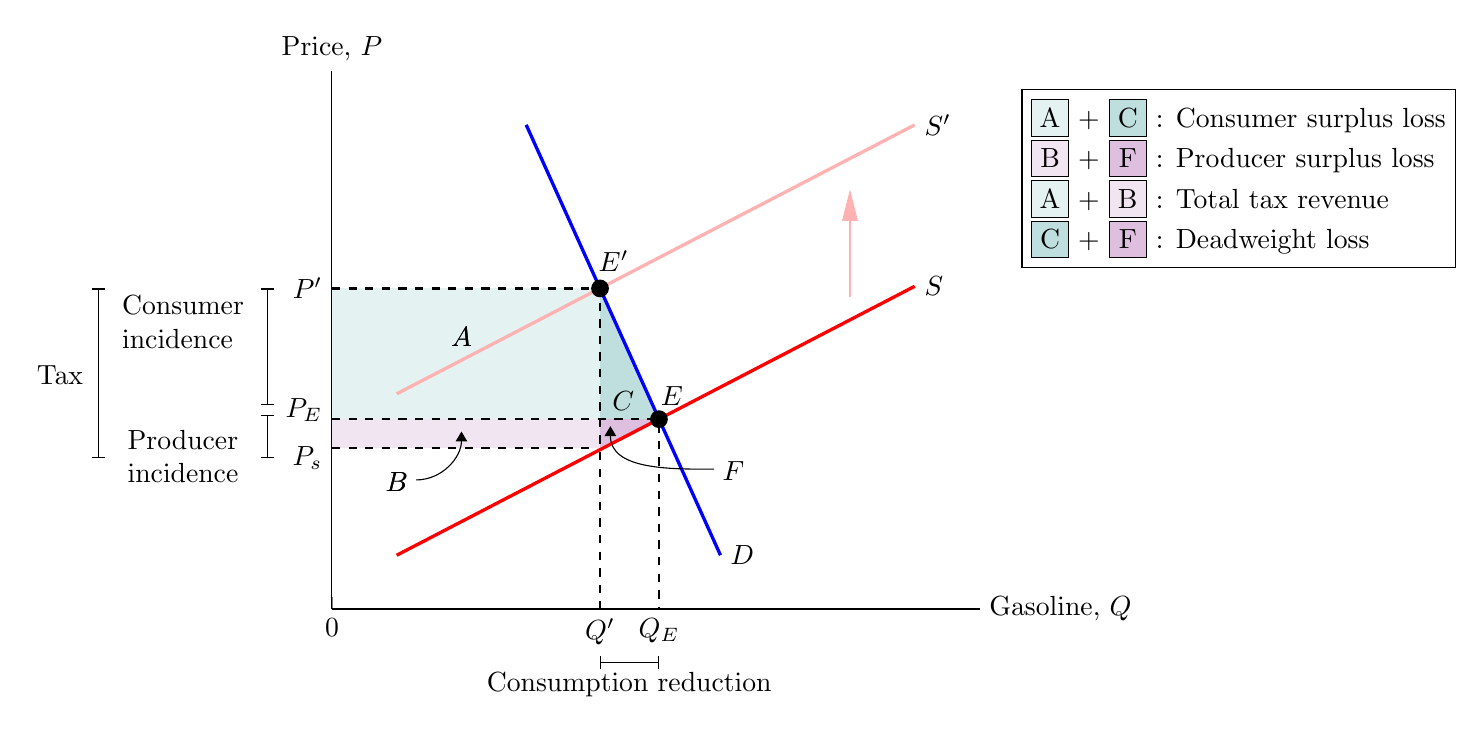
\begin{tikzpicture}
\begin{axis}[
scale = 1.2,
xmin = 0, xmax = 10,
ymin = 0, ymax = 10,
axis lines* = left,
xtick = {0}, ytick = \empty,
axis on top,
clip = false,
]
% Colouring areas
\fill[teal, opacity = 0.1] (0, 3.53) -- (4.14, 3.53) -- (4.14, 5.96) -- (0, 5.96);
\fill[violet, opacity = 0.1] (0, 3.53) -- (4.14, 3.53) -- (4.14, 3) -- (0, 3);
\fill[teal, opacity = 0.25] (4.14, 3.53)-- (5.05, 3.53) -- (4.14, 5.96);
\fill[violet, opacity = 0.25] (4.14, 3)-- (5.05, 3.53) -- (4.14, 3.53);

% Supply and Demand Curves
\addplot[color=blue, very thick] coordinates {(3,9)(6,1)};
\addplot[color=red, very thick] coordinates{(1,1)(9,6)};
\addplot[color=red!30, very thick] coordinates{(1,4)(9,9)};

% Quantity and Price Lines
\addplot[color=black, dashed, thick] coordinates {(0, 5.96)(4.14, 5.96)(4.14, 0)};
\addplot[color=black, dashed, thick] coordinates {(0, 3.53)(5.05, 3.53)(5.05, 0)};
\addplot[color=black, dashed, thick] coordinates {(0, 3)(4.1, 3)};

% Coordinate points
\addplot[color=black, mark=*, only marks, mark size=3pt] coordinates {(4.14, 5.96)(5.05, 3.53)};

% Labels
\node [above] at (5.25, 3.6) {$E$};
\node [above] at (4.35, 6.1) {$E^{\prime}$};

\node [above] at (current axis.above origin) {Price, $P$};
\node [right] at (current axis.right of origin) {Gasoline, $Q$};

\node [right] at (6,1) {$D$};
\node [right] at (9,6) {$S$};
\node [right] at (9,9) {$S^{\prime}$};

\node [above] at (2, 4.7) {$A$};
\node [above] at (1, 2) {$B$};
\node [above] at (4.5, 3.5) {$C$};
\node [above] at (6.2, 2.2) {$F$};

\node [above] at (2, 4.7) {$A$};
\node [above] at (1, 2) {$B$};

\node [left] at (0, 5.96) {$P^{\prime}$};
\node [left] at (0, 3.7) {$P_E$};
\node [left] at (0, 2.8) {$P_s$};

\node [below] at (5.05, 0) {$Q_E$};
\node [below] at (4.14, 0) {$Q^{\prime}$};

\draw[|-|] (4.14, -1) -- (5.05, -1);
\node [below] at (4.59, -1) {Consumption reduction};

\draw[|-|] (-1, 5.96) -- (-1, 3.8);
\node [below, align=left] at (-2.3, 6) {Consumer\\incidence};

\draw[|-|] (-1, 3.6) -- (-1, 2.8);
\node [below, align=left] at (-2.3, 3.5) {Producer\\incidence};

\draw[|-|] (-3.6, 5.96) -- (-3.6, 2.8);
\node [below, align=left] at (-4.2, 4.7) {Tax};

% Arrows
\draw[-{Triangle[length=4mm, width=2mm]}, red!30] (8, 5.8) to (8, 7.8);
\draw[-Triangle] (1.3, 2.4)  to [out = 0, in = 270] (2, 3.3);
\draw[-Triangle] (5.9, 2.6)  to [out = 180, in = 270] (4.3, 3.4);

% Legend
\node[draw, align=left] at (14, 8){
\fcolorbox{black}{teal!10}{\makebox[\fontcharht\font`X]{A}} + \fcolorbox{black}{teal!25}{\makebox[\fontcharht\font`X]{C}} : Consumer surplus loss\\
\fcolorbox{black}{violet!10}{\makebox[\fontcharht\font`X]{B}} + \fcolorbox{black}{violet!25}{\makebox[\fontcharht\font`X]{F}} : Producer surplus loss\\
\fcolorbox{black}{teal!10}{\makebox[\fontcharht\font`X]{A}} + \fcolorbox{black}{violet!10}{\makebox[\fontcharht\font`X]{B}} : Total tax revenue\\
\fcolorbox{black}{teal!25}{\makebox[\fontcharht\font`X]{C}} + \fcolorbox{black}{violet!25}{\makebox[\fontcharht\font`X]{F}} : Deadweight loss
};
\end{axis}
\end{tikzpicture}\hspace*{-3cm}
\end{center}
\textbf{Figure 6-4:} The effect of a gasoline tax on consumption and production and total tax revenue.

\end{document}